\begin{fullwidth}
\chapter{Circuit Quantum Electrodynamics}\label{chap:cQED}
\end{fullwidth}
While many platforms can be used as quantum processors, our focus will be on circuits consisting of superconducting materials. In this chapter, we will go through how these qubits are designed to create qubits and how we can model these numerically. \\

\section{Circuit QED}
\begin{marginfigure}[5 cm]
    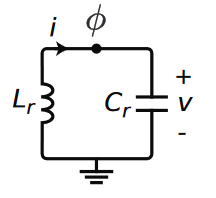
\includegraphics[width = \linewidth]{tex/fig_for_text/LC_circuit.png}
    \caption{Circuit diagram for the LC circuit.}
\end{marginfigure}
Classically, we describe the dynamics of a circuit in terms of its current, $I(t)$, and its voltage drop, $V(t)$. If we consider a simple circuit with one capacitor and one inductor, we have an LC circuit. The energy and subsequent equations of motion are found by summing the energy contributions from each of its elements. The capacitor stores a charge which gives an energy contribution:
\begin{equation}
    E_{\text{capacitor}} = \frac{1}{2} CV^2 = \frac{Q^2}{2C}
\end{equation}
where $Q$ is the charge on the capacitor and $C$ is the capacitance related to the distance between two capacitance plates, the area and the permittivity of the material. We can relate the charge in the capacitor to the current by $Q(t) = Q(t_0) + \int_{t_0}^{t} dt' I(t')$. The other component is an inductor which can take many different form, one example is a coil. The inductor stores energy in a magnetic flux through it, giving an associated energy contribution:
\begin{equation}
    E_{\text{inductor}} = \frac{\Phi^2}{2 L}
\end{equation}
Where $\Phi$ is the flux through the inductor and $L$ is the impendance. If the inductor was a coil, the inducatance would be related to the amount of windings, the permability materials, and its length and area. By using Faradays law, one find a relation between the current drop over the inductor and its flux: $\Phi(t) = \Phi(t_0) + \int_{t_0}^t V(t')dt'$. The total energy of the LC circuit is now \cite{blais_circuit_2021}:
\begin{equation}
    \mathcal{H} = \frac{1}{2C} Q^2 + \frac{1}{2L} \Phi^2
\end{equation}
Which is of particular interest since $Q$ is a canonical momentum to the coordinate $\Phi$\sidenote[][-4cm]{To see this, we can rewrite the capacitor energy in terms of the flux: $\frac12 C \dot \Phi^2$ and define the lagrangian as the difference between kinetic and potential energy: $\mathcal{L} = E_{\text{capacitor}} - E_{\text{inductor}}$. Differentiating the Lagrangian with respect to the time-derivative of flux, we find $\frac{\partial}{\partial\dot{\Phi}} \mathcal{L} = Q$. \cite{krantz_quantum_2019}}. 




% The dynamics can then be calculated using the Lagrange formalism, where we find define the flux:
% \begin{equation}
%     \Phi (t) = \int_{-\infty}^t V(t')dt'
% \end{equation}
% Now using this relations together with $V = L dI/dt$ and $I = C dV/dt$ it is possible to find the energy by:
% \marginnote[0.5 cm]{The lower integration limit comes from the assumption that the system was at rest at infinity}
% \begin{equation}\label{eq: Energy from current and voltage}
%     E(t) = \int_{-\infty}^t V(t')I(t')dt'
% \end{equation}
% Such that the energy of the components are:
% \begin{equation}
%     E_{capacitor} = \frac12 C \dot{\Phi}^2; \quad E_{inductor} = \frac{1}{2L} \Phi^2
% \end{equation}
% Defining the capacitant energy as the kinetic energy $T_C$ and inductive energy as $U_L$, we can write the Lagrangian as:
% \begin{equation}
%     \mathcal{L} = T_C - U_L = \frac12 C \dot{\Phi}^2 - \frac{1}{2L} \Phi^2
% \end{equation}
% And from this the Hamiltonian:\footnote{By defining a canonical momentum $Q = \partial \mathcal{L} / \partial \dot{\Phi}$ and doing the legendre transformation $\mathcal{H} = Q\dot{\Phi} - \mathcal{L}$.} \cite{krantz_quantum_2019}:

\subsection{Going quantum}
 Usually, classical circuits exhibit energy loss due to the resistance in the material. By utilizing the superconducting phase of materials where they exhibit no loss at cold temperatures, circuits can have no energy dissipation\footnote{at least not through resistance. Many other outside factors can still interact with the qubit. The limited coherence is still a big obstacle for superconducting qubit.}. This allows us to quantize the variables and use the superconducting circuit as a type of artificial atom. \cite{superconduting}

Since $\Phi$ and $Q$ are conjugate variables, they satisfy the classical Poisson bracket equation:
\begin{equation}
    \{ \Phi, Q\} = \pfrac{\Phi}{\Phi}\pfrac{Q}{Q} - \pfrac{\Phi}{Q}\pfrac{Q}{\Phi} = 1
\end{equation}
Quantizing these parameters are done by replacing the variables with the corresponding operators: $Q \to \hat{Q}$ and $\Phi \ \to \phi$, and applying the correspondence principle. Here we replace the Poisson brackets with the commutator $\{., .\} \to i\hbar[., .]$, such that operators satisfy \cite{krantz_quantum_2019}:
\begin{equation}
    [\phi, \hat{Q}] = i\hbar
\end{equation}
The rest of this thesis will concern quantum mechanics, so we drop the hats from the operators and set $\hbar = 1$. We can reintroduce it later if we need to determine physical quantities. However, we will often refer to energies in terms of the associated frequency $f = \omega/2\pi = E / h$. 

\subsection{Solving the LC Circuit}\label{sec:forming_qubits}
Since $Q$ and $\Phi$ are conjugate variables like position $x$ and momentum $p$, we can choose to represent it in the flux basis. Here $Q$ takes a differential form:
\begin{equation}
    Q = i\frac{\partial}{\partial \Phi}
\end{equation}
The LC circuit Hamiltonian becomes:
\begin{equation}
    H \ket{\psi} = - \frac{1}{2C} \pfracsquared{}{\Phi}\ket{\psi} + \frac{1}{2L} \Phi^2 \ket{\psi}
\end{equation}
This is exactly the form of a particle in a harmonic potential and we can follow the same procedure and introduce the ladder operators $a, a^\dagger$. Such that the the Hamiltonian can be written as:
\begin{equation}
    H = \omega \left(a^\dagger a + \frac12\right)
\end{equation}
Where $\omega = \sqrt{8 E_C E_L}$ can be found by comparing the Hamiltonian with the one from the harmonic oscillator.

While the harmonic oscillator has many useful properties, a major problem is its equidistant energy levels. When driving transitions with a pulse of frequency $\omega$, we will not only drive transitions in the computational basis $\ket{0} \leftrightarrow\ket{1}$, but also to the higher order states. To find a circuit, we can control without going out of the computational basis, we must search for an anharmonic potential \cite{lc_circuit}.

\section{Building Qubits}
The solution lies in another component, which is exists in the realms of superconducting circuits. By separating two superconductors by a semiconducting material, the Cooper pairs\footnote{Superconductivity is often modelled by creating electron pairs which then have spin 1 and behave like bosons. These pairs are called Cooper pairs. \cite{BCS}} will no longer travel without resistance through the semi conductor but instead tunnel through. The probability of tunneling is dependent on the distance, material and most importantly the phase difference between the two superconductors. The probability for tunneling through the superconducting phase is given as $\sin(2e\phi(t))$, where $\phi(t)$ is the time-dependent difference in phase between the two superconductors. Using the flux-quantum $\phi_0 = h / 2e$ and adding an external flux, the current through the Josephson Junction is:
\begin{equation}
    I(t) = I_0 \sin \left( \frac{\phi(t) + \phi_{ext}}{\phi_0} \right)
\end{equation}
The energy of the Josephson Junction can now be found to\cite{krantz_week_2019}: 
\begin{equation}
    E_{\text{Josephson Junction}} = - E_J \cos \left[ \frac{\phi(t) + \phi_{ext}}{\phi_0} \right]
\end{equation}
up to a constant, which can be neglected by moving the zero point of the energy. \cite{vool_introduction_2017}

\subsection{The Cooper Pair Island}
Replacing the inductor in the LC circuit with a Josephson Junction, we get a circuit with a non-quadratic potential. The Hamiltonian is given by:
\begin{marginfigure}
    \caption{An example of a circuit with a capacitor and a Josephson Junction}
    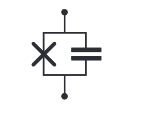
\includegraphics[width = \textwidth]{tex/fig_for_text/CooperPairIsland.png}
    \label{fig:cooper_pair_island}
\end{marginfigure}

\begin{equation}
    H(t) =  4 E_C (n - n_g)^2 -  E_J \cos \left[ \frac{\phi(t) + \phi_{ext}}{\phi_0} \right]
\end{equation}
where $n = Q/2e$ is a amount of cooper pairs on the "island" and $E_C = e^2/2C$\footnote{The factor of 4 would disappear if we counted electrons instead of pairs which was historically done}. Like flux and charge, the Cooper Pair number $n$ and the superconducting phase difference $\phi$ form a canonical commutation pair: $\comm{n}{\phi} = i$. In the Cooper Pair Box the energy scales of the two contributions are approximately equal $E_C \approx E_L$ \cite{blais_circuit_2021}. 


\begin{figure}
    \centering
    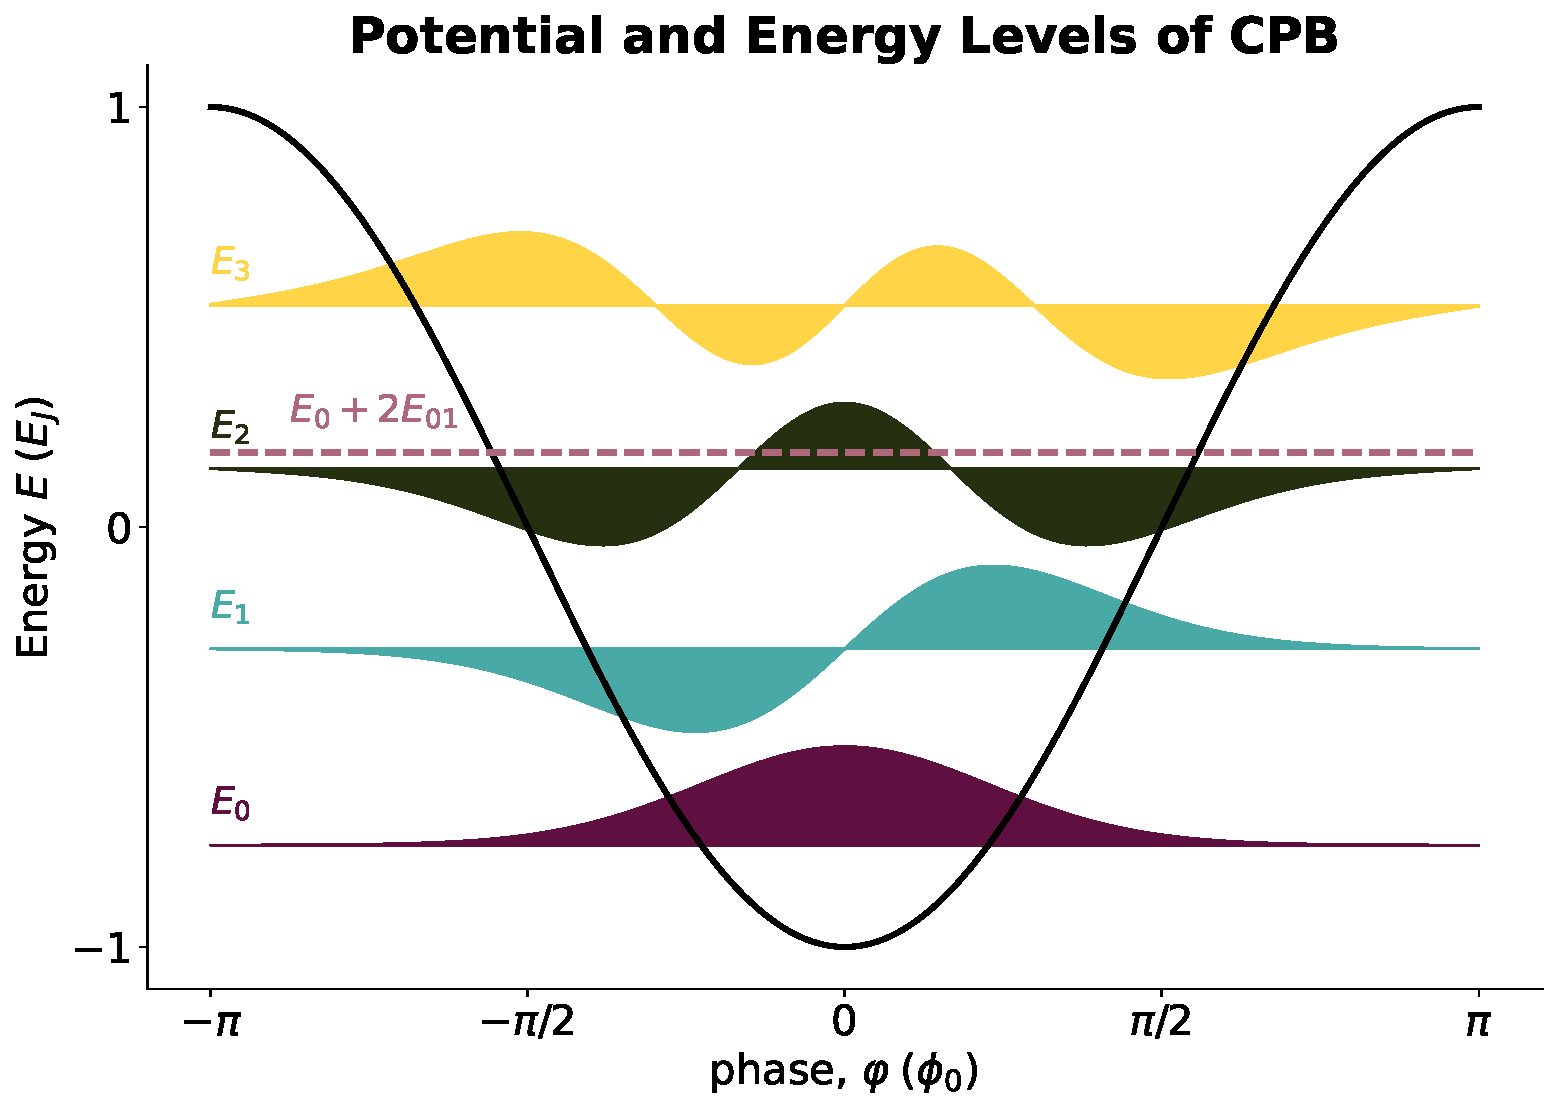
\includegraphics[width=0.80\linewidth]{Figs/Theory/CPB_potential.pdf}
    \caption{The flux-potential of the cooper pair box along with the three lowest energy eigenstates. The eigenstates are shifted according to the theiry energy and scaled to improve readability. The energy level $E_0 + 2E_{01}$ is shown for comparison. The anharmonicity will be the difference between that line and the $E_2$}
    \label{fig:cooper_pair_box_energy_levels}
\end{figure}


This allows us to think about $\phi$ as a coordinate where the Josephson Junction energy defines a potential and the charge a kinetic energy. Solving the eigenvaue problem $H\psi(\phi) = E \psi(\phi)$, we can find the eigenenergies and the eigenvectors of the Cooper Pair Island in $\phi$-space. A solution to this problem with $E_C = E_L$ can be seen in figure \ref{fig:cooper_pair_box_energy_levels}. Most importantly, we note that the that the energy $E_2-E_1 \neq E_1 - E_0$. This difference is called \textit{anharmonicity} and is defined by $\alpha = (E_2 - E_1) - (E_1 - E_2)$ \cite{krantz_week_2019}.

\subsection{The Transmon}
With $E_J / E_C \approx 1$ the circuit is susceptible to charge noise, where small variations change the energy significantly. Charge noise is is harder to control than flux noise, so the superconducting community has moved toward higher ratios for $E_J / E_C$. Most commonly the ratio is somewhere between 50 and 100. By plotting the energy levels of the cooper pair box and the Transmon as function of $n_g$, we can see the difference (see figure \ref{fig:transmon_charge_sensitivity}. The insensitivity to charge noise does not come for free but reduces the anharmonicity. With lower anharmonicity, we need longer pulses to make sure, we do not accidental have components of the $E_2 - E_1$ frequency in our pulse, but the wide use of the Transmon indicates that it strikes a good balance \cite{koch_charge_2007}. 
\begin{marginfigure}
    \centering
    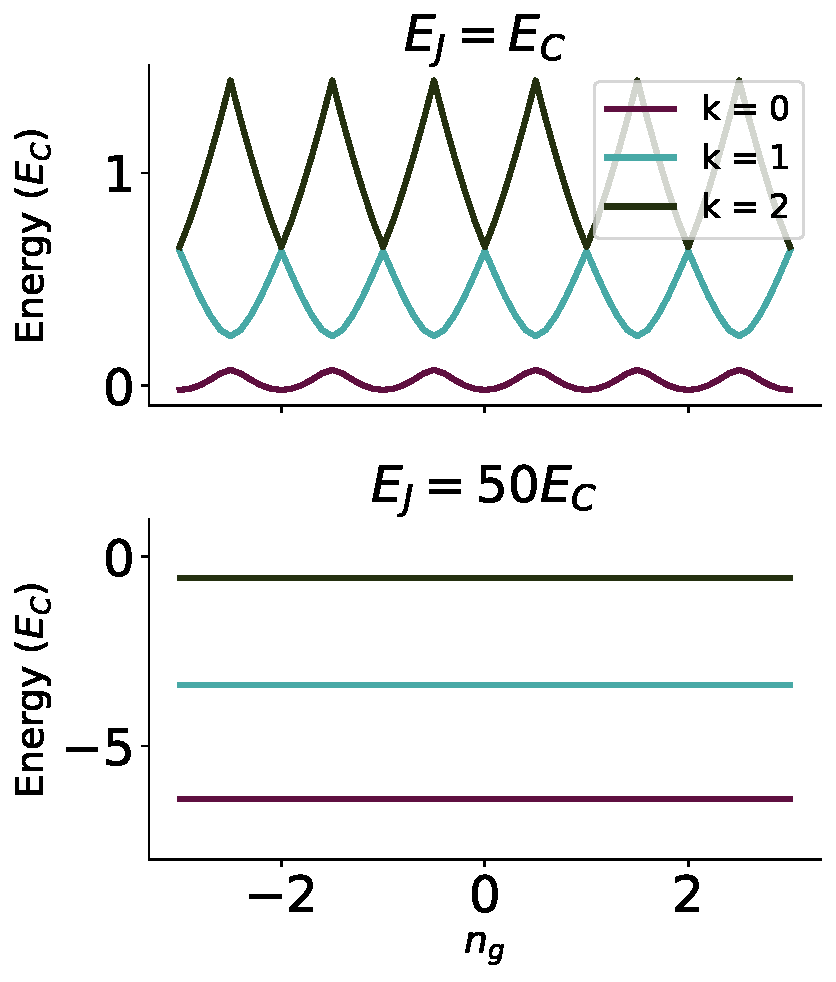
\includegraphics[width = 1.00 \linewidth]{Figs/Theory/Transmon_energy_vs_ng.pdf}
    \caption{The energy levels of the Transmon at different levels of $E_J / E_C$.}
    \label{fig:transmon_charge_sensitivity}
\end{marginfigure}

Multiple additions can be made to the Transmon to make its energy tuneable. A possibility is to alter the Josephson Junction with a loop of two. This creates a SQUID, where the flux through the loop can adjust the energy levels of the circuit \cite{blais_circuit_2021}. 



\section{Numerical cQED}
To simulate the devices considered in this thesis, we will in this section introduce how the problems at hand can be represented in a suitable way for solving numerically. As mentioned in the previous sections, the Hamiltonian is made out of the two conjugate operators $\phi$ and $n$ satisfying the commutation relation $\comm{\phi}{n} = i$. Like the position and momentum, we now have a choice of which basis to represent the system in. In mechanical quantum problem, we would for example consider the position basis ${x}$ and the momentum $p$. These two basis are related by Fourier transformations, and we get\footnote{This is very similar to the relation between $x$ and $p$, but with the extra detail that $n$ is discrete and $\phi\in[0, 2\pi]$}  \cite{langford_circuit_2013}:
\begin{align}
    \ket{\phi} &= \sum_{n=-\infty}^\infty e^{in\phi}\ket{n} \\
    \ket{n} &= \frac{1}{2\pi} \int_0^{2\pi}d\phi e^{-in\phi}\ket{\phi}
\end{align}
Often the problem at hand is easier to formulate in one basis rather than the other. For the transmon, the charge is often localized around $0$ since higher $n- n_g$ values give very high energies. Since the occupation in the higher levels will be negligible if we control the system properly and keep it at low temperatures, we can set a value for $n_{\text{cutoff}}$ to have a finite size of the Hilbert Space. The charge basis is proportional to $n$, so we can use that as basis, where $n$ becomes:
\begin{equation}
    \hat{n} = \begin{pmatrix}
-n_{\text{cutoff}} & 0 &  & \ldots &  \\
0 & -n_{\text{cutoff}}+1 &  &  &  \\
 &  & \ddots &  &  \\
\vdots &  &  & n_{\text{cutoff}}-1 &  \\
 &  &  &  & n_{\text{cutoff}} 
\end{pmatrix}
\end{equation} 
% \end{fullwidth}
To represent the full Hamiltonian we also need $\cos(\phi / \phi_0)$ in the charge basis. Here we will use that:
\begin{align*}
    e^{\pm i \phi}\ket{n} &=  \frac{1}{2\pi} \int_0^{2\pi} d \phi' e^{-in\phi'} e^{\pm i \phi}\ket{\phi'} \\
                          &=  \frac{1}{2\pi} \int_0^{2\pi} d \phi' e^{-i\phi'(n\pm 1)} \ket{\phi'} = \ket{n\mp 1}    
\end{align*}
Since it is true for all states that the operator $e^{i\phi}$ takes a state $\ket{n}$ to $\ket{n+1}$, we can write it in charge basis as:
\begin{equation}
    e^{i\phi} = \sum_n \ket{n}\bra{n+1}; \quad e^{-i\phi} = \sum_n  \ket{n}\bra{n-1}
\end{equation}
Just rewriting cosine in terms of the Euler into complex exponentials, we find 
% \begin{fullwidth}
\begin{align}
    \cos(\phi/\phi_0 + \phi_{ext}) &= \frac12 \left(e^{-i(\phi/\phi_0 + \phi_{ext})} + e^{i(\phi/\phi_0 + \phi_{ext}}))\right) \nonumber\\
    &= \frac12 \left(e^{i\phi_{ext}}e^{i\phi/\phi_0} + e^{-i\phi_{ext}}e^{-i\phi/\phi_0}\right)  \nonumber \\
    &= \frac12 \sum_n \left(e^{i\phi_{ext}} \ket{n}\bra{n + 1} + e^{-i\phi_{ext}} \ket{n}\bra{n+ 1}   \right) \nonumber \\
    &= \frac12 \begin{pmatrix}
        0 & e^{-i\phi_{ext}} & 0 & \hdots \\
        e^{i\phi_{ext}} & 0 & e^{-i\phi_{ext}} \\
        0 & e^{i\phi_{ext}} & 0 & \\
        \vdots & & & \ddots 
    \end{pmatrix}
\end{align}
% \end{fullwidth}
With no external flux, $\phi_{ext} = 0$, this reduces to a matrix with $\frac12$ on the off-diagonals.

Some problems are more convenient to represent in the flux basis. Here we would take the flux to be the diagonal representation, where the diagonal is $(-\pi, -\pi + \delta \dots, \pi)$. $n$ would take a discrete form of the differential $i\pfrac{}{\phi} \approx \frac{i}{2\delta} \sum_k (\ket{-\pi + k\delta}\bra{\pi} + \ket{\pi}\bra{-\pi + k\delta})$ \cite{aumann_circuitq_2022}.

With a Hamiltonian represented in a discrete basis, we can calculate the eigenvalues and eigenvectors numerically. We can further reduce the size of the Hilbert space, by representing it in the energy eigenbasis. Here we just include the few lowest energy levels, and can calculate the representation of for example $n$ by $\mel{k}{q}{k}$. % By limiting us to the few lowest energy eigenstates because of the low temperature, we can reduce the basis significantly to the energy representation, where the Hamiltonian is diagonal: $H = \sum_k^{k_{max}} \hbar \omega_k \ket{k}\bra{k}$ where $k$ refers to the k'th lowest energy eigenvalue of the Hamiltonian. We can then further find the charge matrix as 


% \textbf{Rambling now. Tighten the following: from . The part with }

% When considering the circuits like the transmon with $\frac{E_C}{E_J}\approx 50$ the dominating term in the hamiltnonian will be the contribution from the charge offset proportional to $(\hat{n} - n_g)^2$. This is a good indication that the charge matrix would be good choice to contain as much information as possible near the diagonal. In the charge basis the charge matrix simply takes the form:

% where $n_{\text{cutoff}}$ is an appropriately set parameter to limit the size of our hilbert space. With the parameters used, this is normally set around 50-100. \\

% With the choice of $n$ as eigenbasis the operator representation for flux will be $\phi = \pfrac{}{\hat{n}}$ in the continuous basis or for finite dimensional Hilbert space, we have:
% \begin{equation}
%     \phi = 
% \end{equation}

% \textbf{Probably do the transmon in the flux basis? }





% \vspace{2 cm}
% \textbf{This could also be a numerical section between section 2.1 and 2.2 which we can base the cooper pair box on. }
% When using the transmon, we use the energy eigenstates as a computational basis. To figure out, how the energy splitting and reactions to charge are, we need to find these energy eigenenergies and states.

% \begin{itemize}
%     \item Start with charge basis
%     \item We can now represent the flux as a potential
%     \item Solving numerically gives lowest eigenenergy and states
%     \item Calculating certain matrix elements between the eigenstates givers us the charge-matrix, flux-matrix, etc.. 
% \end{itemize}


% \section{Experimental Setup}
% While most of the work in this thesis will be theoretical and computational, we will try to understand, calibrate and model a physical system. This section will serve as a short overview of the setup.
% % \todo{Write this section properly.}

% \subsection{Soprano Chip}
% The experiments are run on the Soprano 6 qubit Chip on qubit ? (see figure \ref{fig:soprano}), a flux tuneable transmon connected to a resonator, drive line and flux line to tune the transmon. The resonator is connected to a feed line which is further connected to the five other resonators (some through a Purcell filter).

% \begin{figure}[h]
%     \begin{minipage}{0.50\textwidth}
%         \centering
%         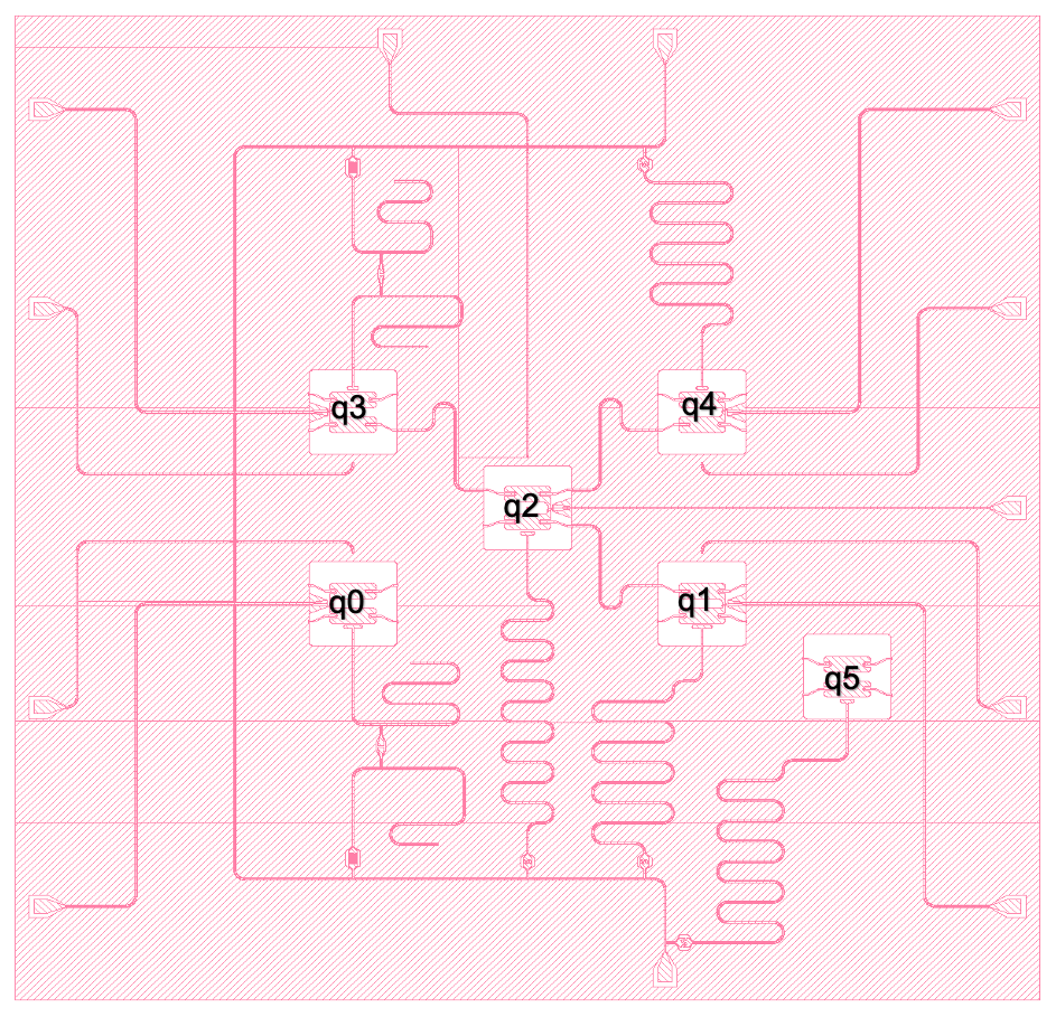
\includegraphics[height = 5 cm]{Figs/hardware/layout.png}
%     \end{minipage}
%         \begin{minipage}{0.50\textwidth}
%         \centering
%         \includegraphics[height = 5 cm]{Figs/hardware/layout_photo.png}
%     \end{minipage}
%     \caption{The Soprano Chip layout and a picture.}
%     \label{fig:soprano}
% \end{figure}

% \subsection{Control Hardware}
% In order to control the qubit and resonator, an arbitrary waveform generator and processing device is used. In this experiment, this is done with an OPX \cite{noauthor_opx_nodate}. The OPX outputs two signals to drive the qubit and one \todo{or two} to the readout line. It has an envelope resolution of 1 GS/s and can process waves with a frequency of 400 MHz. In addition, it is connected with two channels for incoming signal from the readout line which can be demodulated on the onboard FPGA chip. 

% Since the signal needed for qubit and resonator control is of order 5-10 GHz, another device for up- and downconversion is needed. Here, we make use of the Octave \cite{noauthor_octave_nodate}. The Octave has multiple local oscillators for down converting signal one of which support up conversion as well. This one is used for readout, and one of the others are used for qubit control. All signal support IQ mixibng interal IQ mixers allowing us to split the signal. 

% The two devices can be controlled by using accessing an API using Python. For this thesis the higher level module OPX\_Control was used which simplifies writing and running experiment using the OPX and Octave. 

% In addition to the driving lines, a DC line is also coupled directly from the OPX to the fridge to adjust the flux in the qubit. This will be constant for all experiments in the qubit sweet spot, so it will mostly be forgotten. 

% \subsection{Cooling and Amplifiation}
% To keep the soprano chip cold, it is places in a Cryostate capable of cooling to $\approx 30 \text{mK}$ while keeping the chip in vaccum to reduce thermal fluctuations and interactions with the environment. 

% \begin{itemize}
%     \item Down Conversion Line
%     \item Up Conversion Line -> TWPA -> higher temperature amplifiers 
% \end{itemize}



% \begin{figure}
%     \centering
%     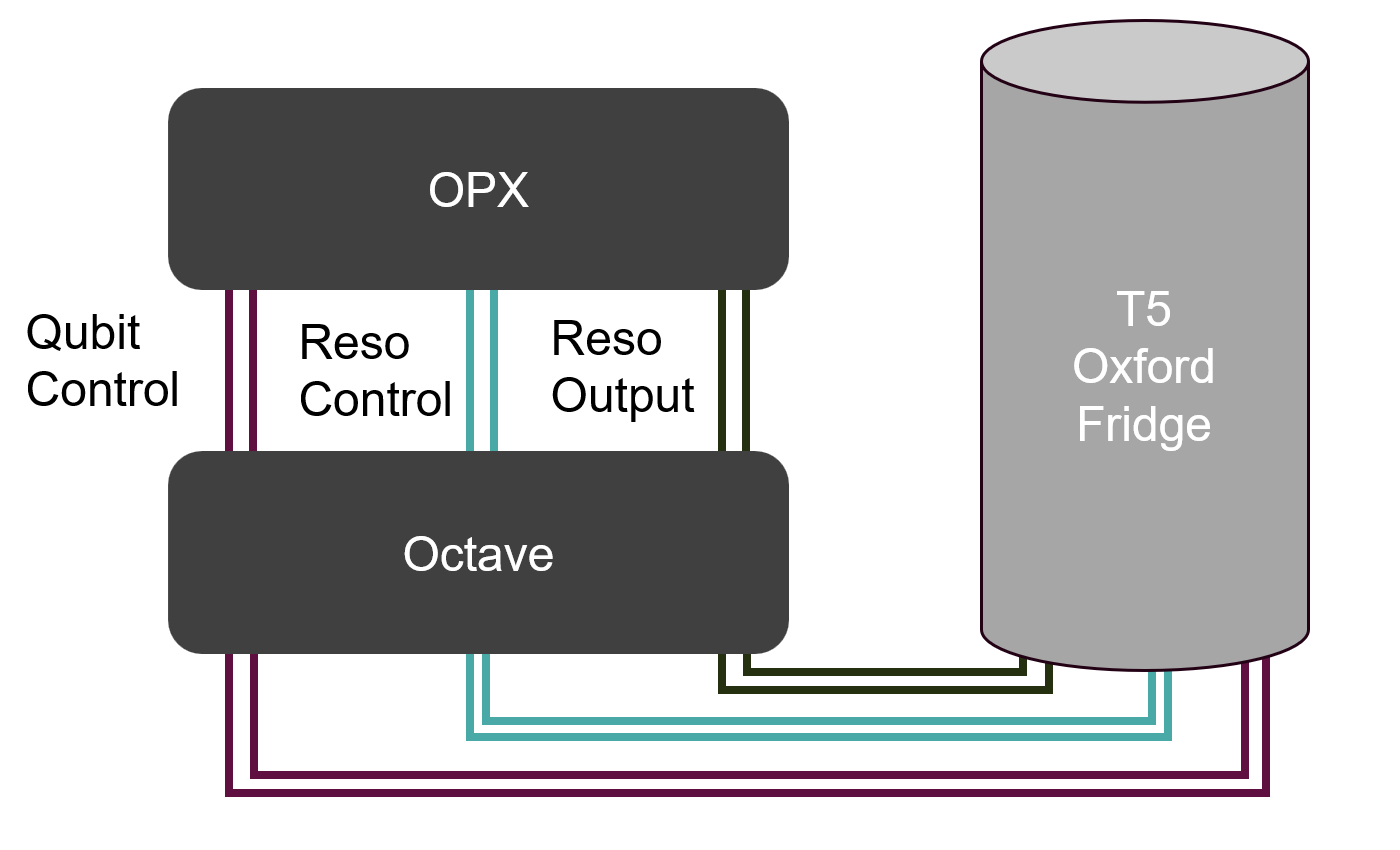
\includegraphics[width=1\linewidth]{Figs//hardware/Setup.png}
%     \caption{A crude schematic of the setup. Qubit control and resonator lines are sent through the octave where they are up converted before going to T5. In the other direction, the signal is downconverted and mixed in the IQ mixer before reentering the OPX where it gets demodulated.}
%     \label{fig:enter-label}
% \end{figure}


% At room temperature the microwave pulses are generated by an Arbitary Waveform Generator in the form of an OPX. The signal from the OPX enters an Octave where it is mixed by an internal local oscillator to convert the microwaves from $\approx 500 \text{ MHz}$ to the suitable $5$ to $10 \text{ GHz}$ before interacting with the qubit or resonator. 

% In the down-conversion line, the readout signal from the cryostate enters the octave, where it enters and IQ mixer splitting the signal in two. After mixing with the local oscillator again it is send back to OPX where it enters a digital to analogue converter before being demodulated and integrated.





